\documentclass[aspectratio=43]{beamer}
\usepackage[latin1]{inputenc}
\usepackage{amsmath}
\usepackage{amsfonts}
\usepackage{amssymb}
\usepackage{makeidx}
\usepackage{graphicx}
\usepackage{array}

% Customization
\mode<presentation>{
\usetheme{CambridgeUS}
\usecolortheme{dolphin}
\setbeamertemplate{navigation symbols}{}
}

%\setbeamertemplate{footline}[frame number]

%TikZ diagrams
\usepackage{tikz}
\usetikzlibrary{patterns}
\usetikzlibrary{arrows,shapes}
\usetikzlibrary{shapes.multipart}
\usetikzlibrary{trees}
\usetikzlibrary{shapes.geometric}
\usetikzlibrary{matrix,arrows}
\usetikzlibrary{positioning}
\usetikzlibrary{calc,through}
\usetikzlibrary{decorations.pathreplacing}
\usepackage{pgffor}

% Define colors
\definecolor{darkgreen}{rgb}{0.0, 0.5, 0.13}
\definecolor{darkblue}{rgb}{0.0, 0.0, 0.55}
\definecolor{darkred}{rgb}{0.55, 0.0, 0.0}

% For using TikZ
\usetikzlibrary{decorations.pathmorphing}
\usetikzlibrary{decorations.markings}
\tikzset{
	vector/.style={decorate, decoration={snake,amplitude=3pt}, draw},
	gluon/.style={decorate, decoration={coil,amplitude=2.5pt},draw},
	provector/.style={decorate, decoration={snake,amplitude=2.5pt}, draw},
	antivector/.style={decorate, decoration={snake,amplitude=-2.5pt}, draw},
	fermion/.style={draw=black, postaction={decorate},
		decoration={markings,mark=at position .55 with {\arrow[draw=black,thick]{>}}}},
	fermionbar/.style={draw=black, postaction={decorate},
		decoration={markings,mark=at position .55 with {\arrow[draw=black,thick]{<}}}},
	fermionnoarrow/.style={draw=black},
	gluon/.style={decorate, draw=black,
		decoration={coil,amplitude=2.5pt, segment length=3pt}},
	gluon2/.style={decorate, draw=black,
		decoration={coil,amplitude=1.75pt, segment length=2.75pt}},
	scalar/.style={dashed,draw=black, postaction={decorate},
		decoration={markings,mark=at position .55 with {\arrow[draw=black]{>}}}},
	scalarbar/.style={dashed,draw=black, postaction={decorate},
		decoration={markings,mark=at position .55 with {\arrow[draw=black]{<}}}},
	scalarnoarrow/.style={dashed,draw=black},
	electron/.style={draw=black, postaction={decorate},
		decoration={markings,mark=at position .55 with {\arrow[draw=black]{>}}}},
	bigvector/.style={decorate, decoration={snake,amplitude=4pt}, draw},
}

% Blocks
\tikzstyle{block} = [draw, rectangle, minimum height = 3em, rounded corners, minimum width = 4em]
\tikzstyle{block2} = [draw, rectangle, minimum height = 3em, rounded corners, minimum width = 7em]
\tikzstyle{circle} = [draw, circle, radius = 1.5]
\tikzstyle{arrow} = [thick,->]
%************************************************************************************************************

% Title and author
\title[ML for PDFs determination]{Machine Learning for the precision determination of Parton Distribution Functions}
\author{\textbf {Jes\'us Urtasun Elizari}}
%\institute{\textbf {University of Milan}}
\date{Milan, September 2019}

\begin{document}

% Front slide
\begin{frame}

	%\maketitle

	\center{\color{blue}Machine Learning for the precision determination of \\Parton Distribution Functions}
	\center{Jes\'us Urtasun Elizari}
	\center{Supervised by Dr.\ Stefano Forte and Dr.\ Stefano Carrazza}
	\center{PhD Seminar - Milan, September 2019}

	\begin{figure}
		\minipage{1\textwidth}
		
\includegraphics[width = 3.0 cm]{unimi.png}
		\hfill
		
\includegraphics[width = 3.0 cm]{n3pdf.png}
		\hfill
		
\includegraphics[width = 3.0 cm]{erc.png}
		\endminipage
	\end{figure}

	\vspace{1.0 cm}
	{ \tiny This project has received funding from the European Union$'$s Horizon 2020 research and innovation program under grant agreement No 740006.}

\end{frame}

% Cartoon
\begin{frame}

	\begin{figure}
		
\includegraphics[width = \linewidth]{joke1.png}
	\end{figure}

\end{frame}

% Cartoon
\begin{frame}

	\begin{figure}
		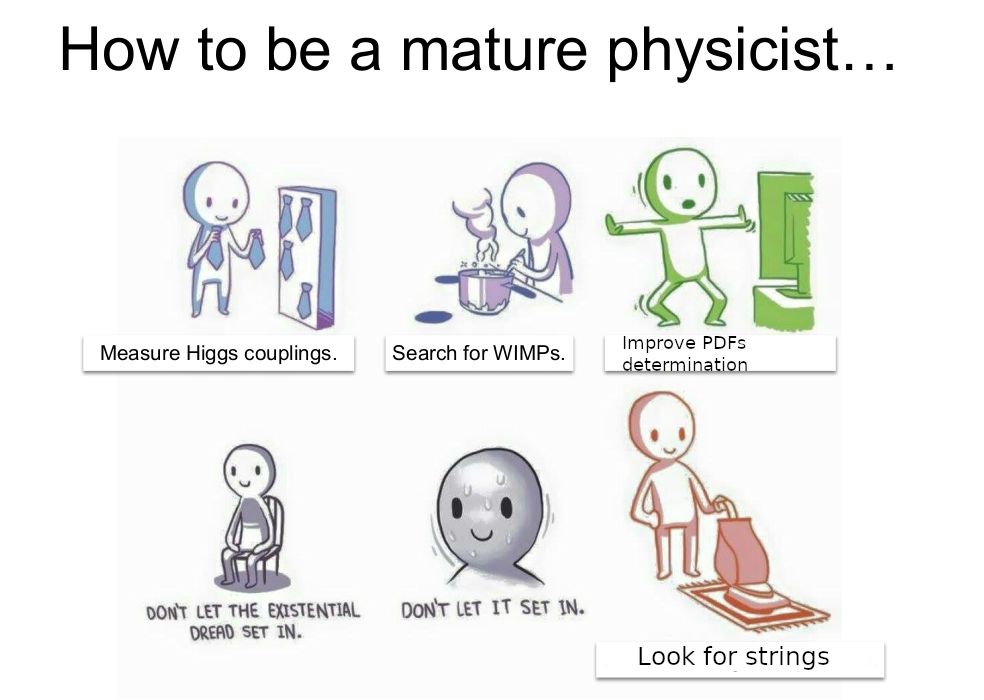
\includegraphics[width = \linewidth]{joke3.png}
	\end{figure}

\end{frame}

% Introduction
\begin{frame}

	\frametitle{Outline}
	
	\begin{enumerate}
		\item {\color{blue}Quantum Chromodynamics in a nutshell}
		\begin{itemize}
			\item The Standard Model
			\item The strong interactions
			\item Parton Distribution Functions
		\end{itemize}
		\item {\color{blue}The N3PDF project}
		\begin{itemize}
			\item Machine Learning for PDFs determination
			\item Operator implementation in TensorFlow
			\item Results $\&$ Conclusions
		\end{itemize}
	\end{enumerate}
	
\end{frame}

% Quantum Chromodynamics in a nutshell
\begin{frame}
	
	\center{\color{blue} Quantum Chromodynamics in a nutshell}

\end{frame}

% The Standard model
\begin{frame}

	\frametitle{Quantum Chromodynamics}
	\framesubtitle{The Standard Model}

	\begin{figure}
		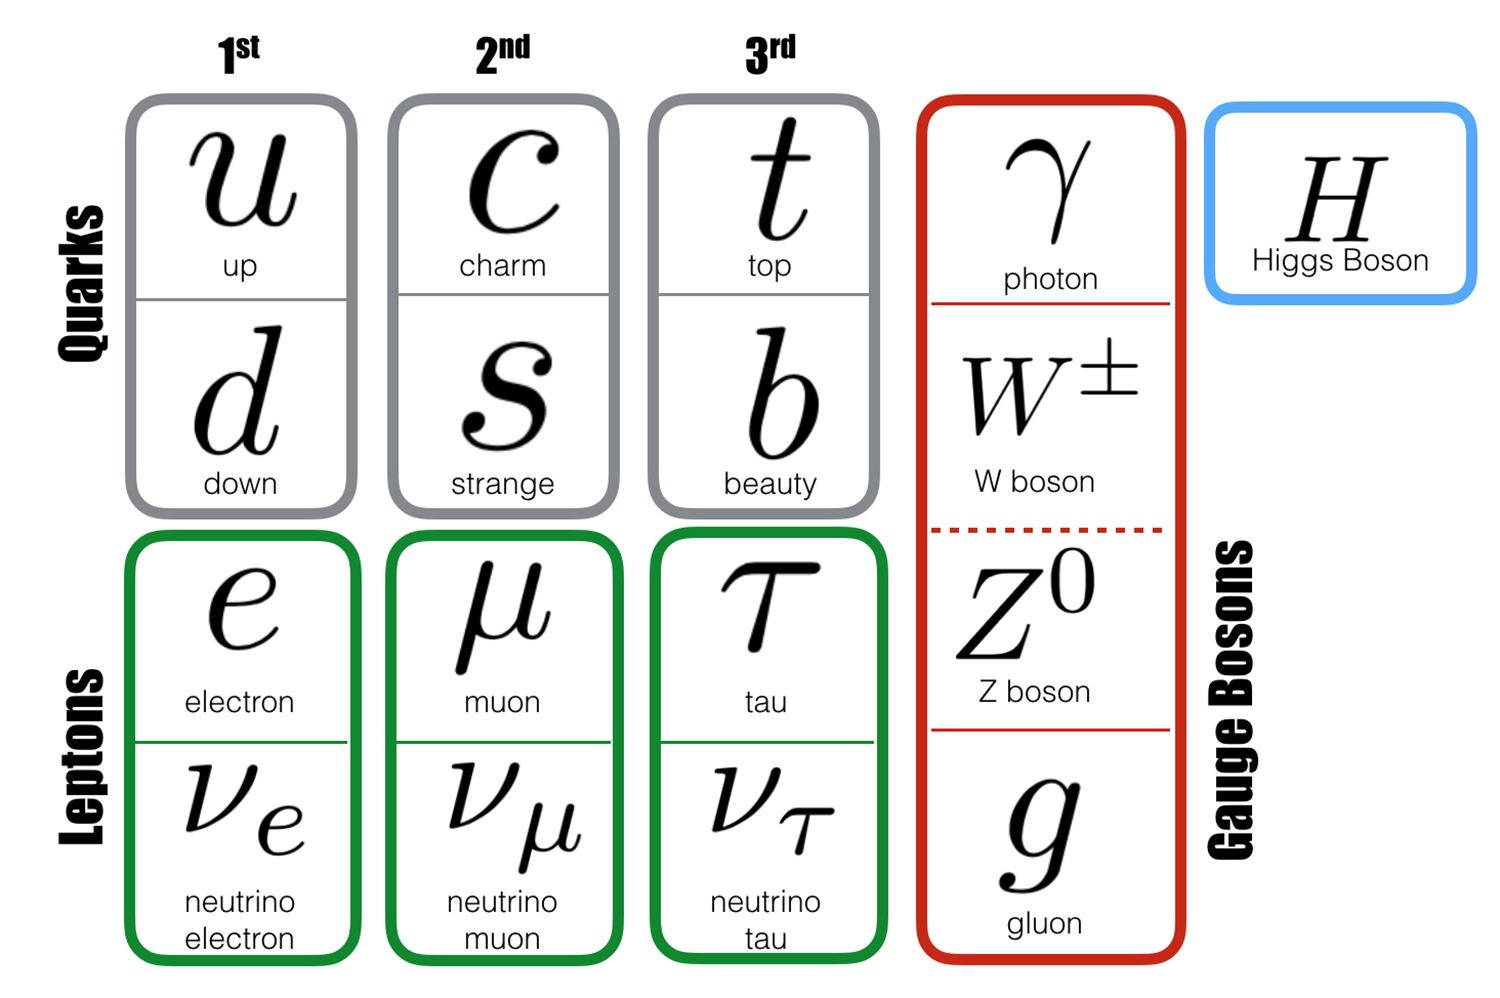
\includegraphics[width = 6 cm]{SM.png}
	\end{figure}
	
	Quantum Field Theory describing physics at the TeV scale
	\begin{enumerate}
		\item Fermions composing matter
		\item Bosons mediating interactions
		\item Scalar Higgs generating mass
	\end{enumerate}
	
\end{frame}

% Explore the proton structure
\begin{frame}

	\frametitle{Quantum Chromodynamics}
	\framesubtitle{Explore the strong interactions}
	
	How to explore proton's inner structure?
	
	\begin{figure}
		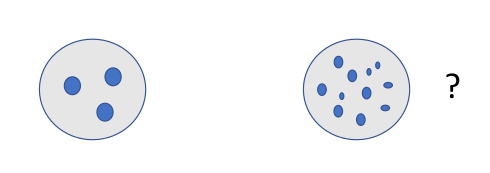
\includegraphics[width = 0.5\linewidth]{protons.png}
	\end{figure}
	
	
	\begin{itemize}
		\item Point-like projectile on the object $\longrightarrow$ DIS
		\item Smash the two objects $\longrightarrow$ LHC physics
	\end{itemize}
	
	{\color{blue}"A way to analyze high energy collisions is to consider any hadron as a composition of point-like constituents $\longrightarrow$ \textbf{partons"} } R.Feynman, 1969 

\end{frame}

% Quantum Chromodynamics and PDFs
\begin{frame}

	\frametitle{Quantum Chromodynamics}
	\framesubtitle{Parton Distribution Functions}
	
	\begin{figure}
		\minipage{0.5\textwidth}
		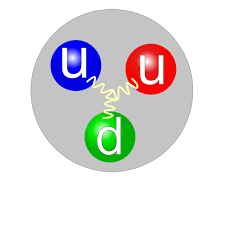
\includegraphics[width = 0.5\linewidth]{proton.png}
		\endminipage\hfill
		\minipage{0.5\textwidth}
		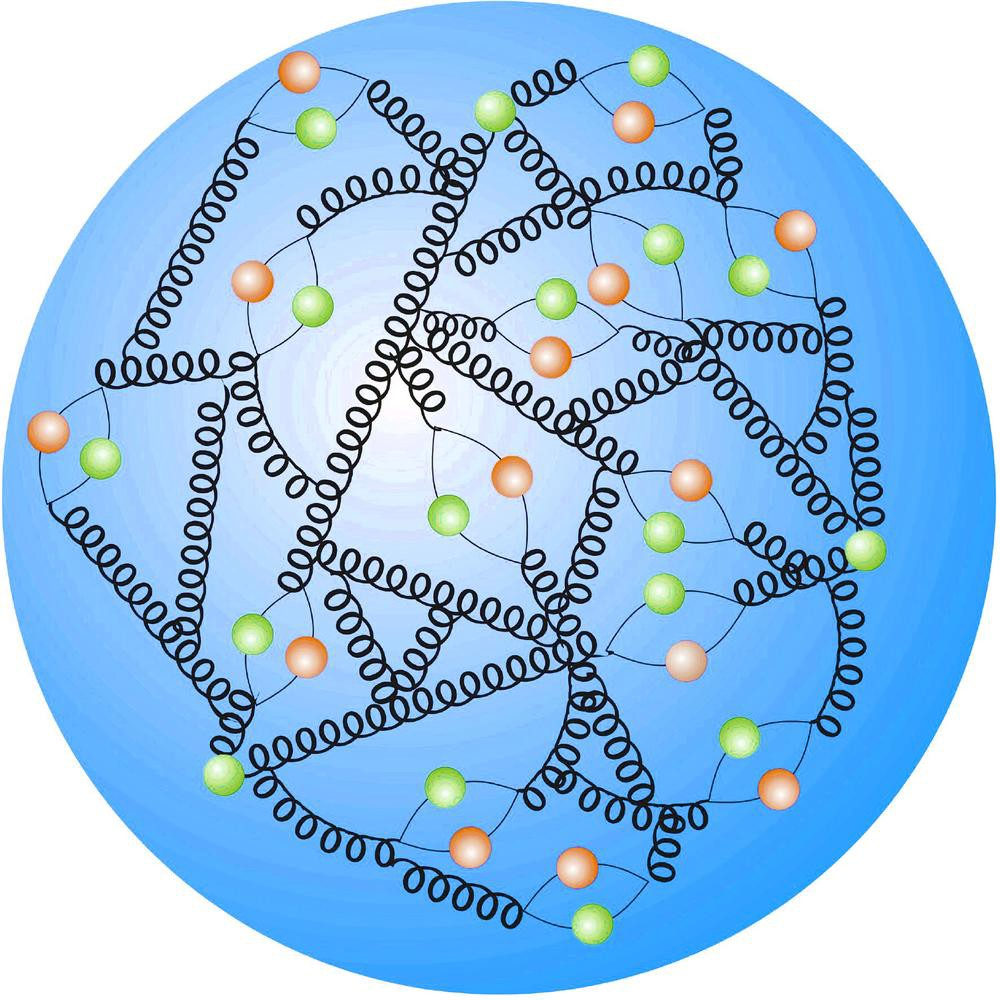
\includegraphics[width = 0.4\linewidth]{proton2.jpg}
		\endminipage
	\end{figure}
	

	\begin{itemize}
		\item Hadrons made of partonic objects $\longrightarrow$ non perturbative physics
		\item Interactions take place only at partonic level
	\end{itemize}

	{\color{blue}Parton Distribution Functions: probability distribution of finding a particular parton (u, d, ..., g) carrying a fraction x of the proton's momentum}

\end{frame}

% Parton Distribution functions
\begin{frame}

	\frametitle{Quantum Chromodynamics}
	\framesubtitle{What PDFs look like}
	
	\begin{figure}
		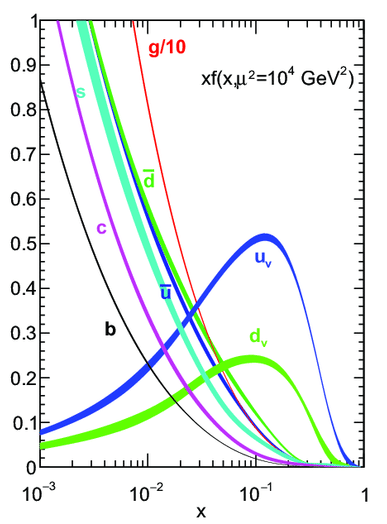
\includegraphics[width = 3.8 cm]{PDF.png}
	\end{figure}
	
	\begin{itemize}
		\item Each parton has a different PDF $\longrightarrow$ ${\color{blue}u(x)}, {\color{green}d(x)}, ..., {\color{red}g(x)}$
		\item PDFs are not predicted, and can not be measured
		\item PDFs are {\color{blue}extracted} from data
	\end{itemize}
\end{frame}

% The N3PDF project
\begin{frame}
	
	\center{\color{blue} The N3PDF project}
	\center{\color{blue} Machine Learning for the precision determination of PDFs}

\end{frame}

% Machine Learning
\begin{frame}

	\frametitle{The N3PDF project}
	\framesubtitle{Machine Learning}
	
	\begin{figure}[!htb]
	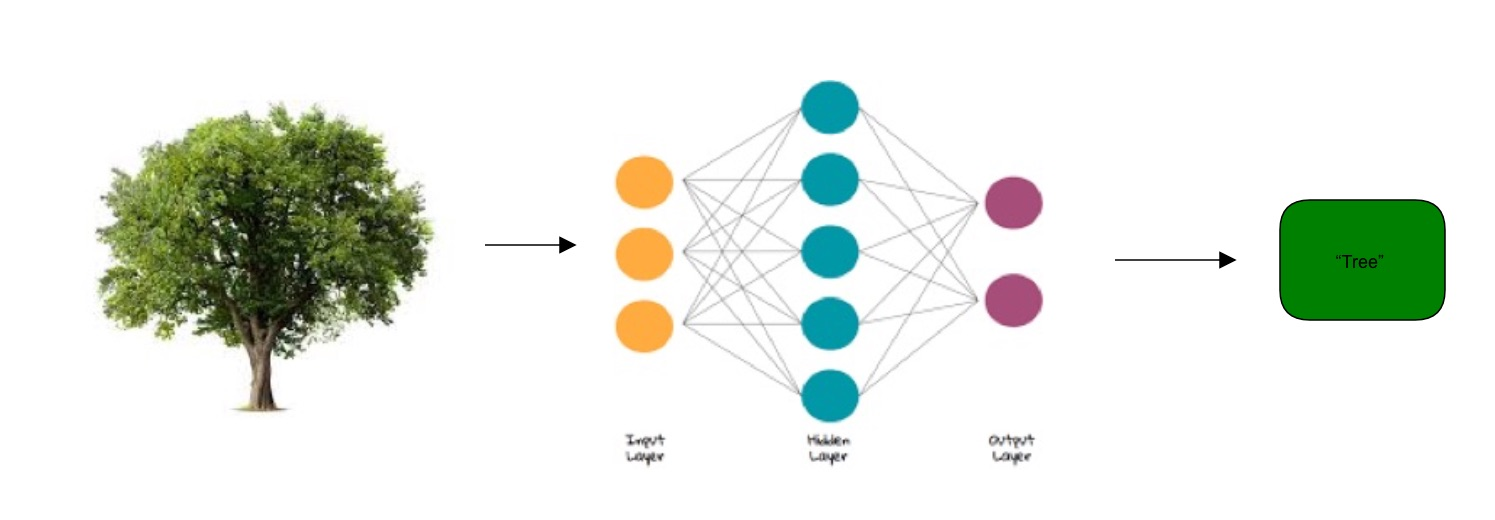
\includegraphics[width = \linewidth]{NNcomplete.jpg}
	\end{figure}
	
	\begin{enumerate}
	\item ML algorithms solve \textit{complex} tasks like classification and regression
	\item Neural Networks $\longrightarrow$ Non linear functions of an input $x$, given by $y(x) = \sigma \{ \textbf{w} \cdot x + b \}$
	\item Rely on comparison with data $\longrightarrow$ \textit{Learning}, need for training $\textbf{w}, b$
	\end{enumerate}

\end{frame}


% What we actually measure
\begin{frame}

	\frametitle{The N3PDF project}
	\framesubtitle{What we actually measure}
	
	Any theory must predict a number $\longrightarrow$ Observable $\sigma$
	
	\begin{figure}
		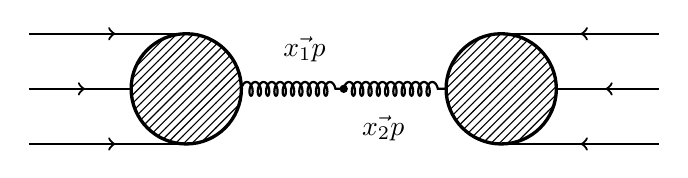
\begin{tikzpicture}
		% Incoming first proton 
		\draw [thick, fermion] (-4, 0.7)--(-2, 0.7);
		\draw [thick, fermion] (-4, 0)--(-2.7, 0);
		\draw [thick, fermion] (-4, -0.7)--(-2, -0.7);
		\draw [thick, very thick, pattern = north east lines] (-2, 0) circle [radius = 0.7];
		% Gluons
		\draw [thick, gluon] (-1.3, 0)--(0, 0);
		\draw [thick, gluon] (0, 0)--(1.3, 0);
		\node at (-0.5, 0.5) {$\vec{x_{1}p}$};
		\node at (0.5, -0.5) {$\vec{x_{2}p}$};
		\draw [thick, very thick, fill = black, pattern = north east lines] (0, 0) circle [radius = 0.03];
		% Incoming second proton
		\draw [thick, very thick, pattern = north east lines] (2, 0) circle [radius = 0.7];
		\draw [thick, fermionbar] (2, 0.7)--(4, 0.7);
		\draw [thick, fermionbar] (2.7, 0)--(4, 0);
		\draw [thick, fermionbar] (2, -0.7)--(4, -0.7);
		\end{tikzpicture}
	\end{figure}
	
	Factorize the problem $\longrightarrow$ Convolute the {\color{red}PDFs}  with the partonic ${\color{blue}\hat{\sigma}_{i j}}$
	
	\begin{equation}
		\sigma = \int_{0}^{1} dx_{1} \; dx_{2} \; {\color{red} f_{\alpha}(x_{1}, \mu_{F}) \ast f_{\beta}(x_{2}, \mu_{F})} \ast {\color{blue}\hat{\sigma}_{\alpha \beta}(\alpha_{s}(\mu_{R}), \mu_{F})} \; \nonumber
	\end{equation}
	
	\begin{itemize}
		\item Use a Neural networks to generate the PDFs
		\item Generate a vector of observables $y_{N}$
	\end{itemize}
	
	\begin{equation}
		y_{N} = \sum_{i, j, \alpha, \beta} {\color{red}f_{\alpha}(x_{i}) \; f_{\beta}(x_{j})} \; {\color{blue}\hat{\sigma}_{N i j \alpha \beta}} \; \nonumber
	\end{equation}

\end{frame}

% General structure of a fit
\begin{frame}

	\frametitle{The N3PDF project}
	\framesubtitle{General structure of n3fit}

	\begin{figure}[!htb]
		\minipage{0.32\textwidth}
		
\includegraphics[width = 0.5\linewidth]{TF.png}
		\endminipage\hfill
		\minipage{0.5\textwidth}
		
\includegraphics[width = 0.5\linewidth]{Keras.png}
		\endminipage\hfill
	\end{figure}

	\begin{itemize}
		\item Use TensorFlow and Keras to determine the PDFs
		\item See paper by S.Carraza - J.Cruz-Martinez \\
		{\color{blue}"Towards a new generation of parton densities\\ with deep learning models",\\ https://arxiv.org/abs/1907.05075}
	\end{itemize}

\end{frame}

% General structure
\begin{frame}

	\frametitle{The N3PDF project}
	\framesubtitle{General structure of n3fit}

	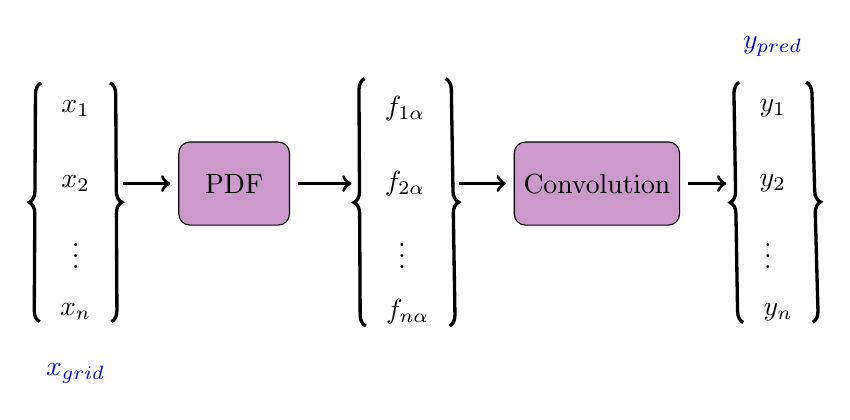
\begin{tikzpicture}
	
	% List of xs
	\node (x1) {$x_{1}$};
	\node[below = 0.5 cm of x1] (x2) {$x_{2}$};
	\node[below = 0.2 cm of x2] (xd) {\vdots};
	\node[below = 0.2 cm of xd] (xn) {$x_{n}$};
	\node[below = 0.3 cm of xn] (xgrid) {\color{blue}$x_{grid}$};
	\coordinate[right = 0.3 cm of x2] (rx2);
	% Braces
	\draw[decorate, decoration={brace, amplitude = 4pt, raise = 1pt}, very thick]
	($(x1.north east) + (0.1, 0.1)$) -- ($(xn.south east) + (0.1, 0.1)$);
	\draw[decorate, decoration={brace, amplitude = 4pt, raise = 1pt}, very thick]
	($(xn.south west) + (-0.1, 0.1)$) -- ($(x1.north west) + (-0.1, 0.1)$);
	
	% PDF layer
	\node[block, fill = violet!40, right = 1.0 cm of x2] (pdf) {PDF};
	\coordinate[left = 0.1 cm of pdf] (lpdf);
	\coordinate[right = 0.1 cm of pdf] (rpdf);
	
	% List of pdfs
	\node[right = 3.5 cm of x1] (f1) {$f_{1 \alpha}$};
	\node[right = 3.5 cm of x2] (f2) {$f_{2 \alpha}$};
	\node[right = 3.8 cm of xd] (fd) {\vdots};
	\node[right = 3.5 cm of xn] (fn) {$f_{n \alpha}$};
	\coordinate[left = 0.3 cm of f2] (lf2);
	\coordinate[right = 0.3 cm of f2] (rf2);
	% Braces
	\draw[decorate, decoration = {brace, amplitude = 4pt, raise = 1pt}, very thick]
	($(f1.north east) + (0.1, 0.1)$) -- ($(fn.south east) + (0.1, 0.1)$);
	\draw[decorate, decoration = {brace, amplitude = 4pt, raise = 1pt}, very thick]
	($(fn.south west) + (-0.1, 0.1)$) -- ($(f1.north west) + (-0.1, 0.1)$);
	
	% Convolution layer
	\node[block, fill = violet!40, right = 1.0 cm of f2] (conv) {Convolution};
	\coordinate[left = 0.1 cm of conv] (lconv);
	\coordinate[right = 0.1 cm of conv] (rconv);
	\coordinate[below = 0.1 cm of conv] (bconv);
	
	% List of y
	\node[right = 4.0 cm of f1] (y1) {$y_{1}$};
	\node[right = 4.0 cm of f2] (y2) {$y_{2}$};
	\node[right = 4.3 cm of fd] (yd) {\vdots};
	\node[right = 4.0 cm of fn] (yn) {$y_{n}$};
	\node[above = 0.3 cm of y1] (ypred) {\color{blue}$y_{pred}$};
	\coordinate[left = 0.3 cm of y2] (ly2);
	% Braces
	\draw[decorate, decoration = {brace, amplitude = 4pt, raise = 1pt}, very thick]
	($(y1.north east) + (0.1, 0.1)$) -- ($(yn.south east) + (0.1, 0.1)$);
	\draw[decorate, decoration = {brace, amplitude = 4pt, raise = 1pt}, very thick]
	($(yn.south west) + (-0.1, 0.1)$) -- ($(y1.north west) + (-0.1, 0.1)$);
	
	% Connect all nodes defined above
	\draw[arrow, very thick] (rx2) -- (lpdf);
	\draw[arrow, very thick] (rpdf) -- (lf2);
	\draw[arrow, very thick] (rf2) -- (lconv);
	\draw[arrow, very thick] (rconv) -- (ly2);
	
	\end{tikzpicture}
	
	\begin{enumerate}
		\item Build a NN to compute $y_{pred}$ observables from a grid $x_{i}$
		\item Compute loss function by comparing with data
		\item Update values of PDF $\longrightarrow$ {\color{violet} Fit}
	\end{enumerate}

\end{frame}

% Operator implementation
\begin{frame}

	\frametitle{The N3PDF project}
	\framesubtitle{Operator implementation}
	
	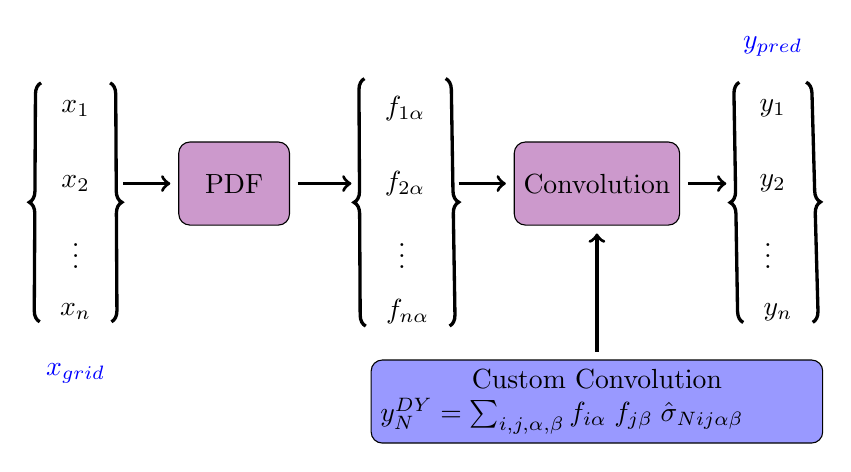
\begin{tikzpicture}
	
		% List of xs
		\node (x1) {$x_{1}$};
		\node[below = 0.5 cm of x1] (x2) {$x_{2}$};
		\node[below = 0.2 cm of x2] (xd) {\vdots};
		\node[below = 0.2 cm of xd] (xn) {$x_{n}$};
		\node[below = 0.3 cm of xn] (xgrid) {\color{blue}$x_{grid}$};
		\coordinate[right = 0.3 cm of x2] (rx2);
		% Braces
		\draw[decorate, decoration={brace, amplitude = 4pt, raise = 1pt}, very thick]
		($(x1.north east) + (0.1, 0.1)$) -- ($(xn.south east) + (0.1, 0.1)$);
		\draw[decorate, decoration={brace, amplitude = 4pt, raise = 1pt}, very thick]
		($(xn.south west) + (-0.1, 0.1)$) -- ($(x1.north west) + (-0.1, 0.1)$);
		
		% PDF layer
		\node[block, fill = violet!40, right = 1.0 cm of x2] (pdf) {PDF};
		\coordinate[left = 0.1 cm of pdf] (lpdf);
		\coordinate[right = 0.1 cm of pdf] (rpdf);
		
		% List of pdfs
		\node[right = 3.5 cm of x1] (f1) {$f_{1 \alpha}$};
		\node[right = 3.5 cm of x2] (f2) {$f_{2 \alpha}$};
		\node[right = 3.8 cm of xd] (fd) {\vdots};
		\node[right = 3.5 cm of xn] (fn) {$f_{n \alpha}$};
		\coordinate[left = 0.3 cm of f2] (lf2);
		\coordinate[right = 0.3 cm of f2] (rf2);
		% Braces
		\draw[decorate, decoration = {brace, amplitude = 4pt, raise = 1pt}, very thick]
		($(f1.north east) + (0.1, 0.1)$) -- ($(fn.south east) + (0.1, 0.1)$);
		\draw[decorate, decoration = {brace, amplitude = 4pt, raise = 1pt}, very thick]
		($(fn.south west) + (-0.1, 0.1)$) -- ($(f1.north west) + (-0.1, 0.1)$);
		
		% Convolution layer
		\node[block, fill = violet!40, right = 1.0 cm of f2] (conv) {Convolution};
		\coordinate[left = 0.1 cm of conv] (lconv);
		\coordinate[right = 0.1 cm of conv] (rconv);
		\coordinate[below = 0.1 cm of conv] (bconv);
		
		% Custom Convolution 
		\node[block, fill = blue!40, below = 1.7 cm of conv, text width = 5.5 cm] (myconv) {\centering Custom Convolution \\ $y_{N}^{DY} = \sum_{i, j, \alpha, \beta} f_{i \alpha} \; f_{j \beta} \; \hat{\sigma}_{N i j \alpha \beta}$};
		\coordinate[above = 0.1 cm of myconv] (amyconv);
		
		% List of y
		\node[right = 4.0 cm of f1] (y1) {$y_{1}$};
		\node[right = 4.0 cm of f2] (y2) {$y_{2}$};
		\node[right = 4.3 cm of fd] (yd) {\vdots};
		\node[right = 4.0 cm of fn] (yn) {$y_{n}$};
		\node[above = 0.3 cm of y1] (ypred) {\color{blue}$y_{pred}$};
		\coordinate[left = 0.3 cm of y2] (ly2);
		% Braces
		\draw[decorate, decoration = {brace, amplitude = 4pt, raise = 1pt}, very thick]
		($(y1.north east) + (0.1, 0.1)$) -- ($(yn.south east) + (0.1, 0.1)$);
		\draw[decorate, decoration = {brace, amplitude = 4pt, raise = 1pt}, very thick]
		($(yn.south west) + (-0.1, 0.1)$) -- ($(y1.north west) + (-0.1, 0.1)$);
			
		% Connect all nodes defined above
		\draw[arrow, very thick] (rx2) -- (lpdf);
		\draw[arrow, very thick] (rpdf) -- (lf2);
		\draw[arrow, very thick] (rf2) -- (lconv);
		\draw[arrow, very thick] (rconv) -- (ly2);
		\draw[arrow, very thick] (amyconv) -- (bconv);
		
	\end{tikzpicture}
	
	\begin{enumerate}
		\item TF relies in symbolic computation $\longrightarrow$ High memory usage
		\item Implement c++ operator replacing the convolution
	\end{enumerate}

\end{frame}

% Results DIS ratio
\begin{frame}

	\frametitle{Results}
	\framesubtitle{Checking computation}
	
	{\Large DIS:}
	\begin{table}
		\centering
		\begin{tabular}{c c c c}
			& TensorFlow & Custom & Ratio \\ \hline
			& 1.9207904 & 1.9207904 & {\color{darkgreen} 1.0000000} \\
			Convolution & 2.4611666 & 2.4611664 & {\color{darkgreen} 0.9999999} \\
			& 1.3516952 & 1.3516952 & {\color{darkgreen} 1.0000000} \\
			\hline
			& 1.8794115 & 1.8794115 & {\color{darkgreen} 1.0000000} \\
			Gradient & 1.505316 & 1.505316 & {\color{darkgreen} 1.0000000} \\
			& 2.866085 & 2.866085 & {\color{darkgreen} 1.0000000} \\
			\hline
		\end{tabular}
	\end{table}

\end{frame}

% Results hadronic ratio
\begin{frame}

	\frametitle{Results}
	\framesubtitle{Checking computation}
	
	{\Large Hadronic:}
	\begin{table}
		\centering
		\begin{tabular}{c c c c}
			& TensorFlow & Custom & Ratio \\ \hline
			& 8.142365 & 8.142366 & {\color{darkgreen} 1.0000001} \\
			Convolution & 8.947762 & 8.947762 & {\color{darkgreen} 1.0000000} \\
			& 7.4513326 & 7.4513316 & {\color{darkgreen} 0.9999999} \\
			\hline
			& 18.525095 & 18.525095 & {\color{darkgreen} 1.0000000} \\
			Gradient & 19.182995 & 19.182993 & {\color{darkgreen} 0.9999999} \\
			& 19.551006 & 19.551004 & {\color{darkgreen} 0.9999999} \\
			\hline
		\end{tabular}
	\end{table}
	
\end{frame}

% Results memory
\begin{frame}

	\frametitle{Results}
	\framesubtitle{Memory saving}

	{\Large Hadronic only:}
	\begin{table}
		\centering
		\begin{tabular}{c c c c}
			& TensorFlow & Custom Convolution & Diff \\ \hline
			Virtual & {\color{red} 17.7 GB} & {\color{darkgreen} 13.8 GB} & {\color{darkgreen} 3.9 GB} \\
			RES & {\color{red} 12.1 GB} & {\color{darkgreen} 8.39 GB} & {\color{darkgreen} 3.2 GB} \\ \hline
		\end{tabular}
	\end{table}
	
	\hfill

	{\Large Global:}
	\begin{table}
		\centering
		\begin{tabular}{c c c c}
			& TensorFlow & Custom Convolution & Diff \\ \hline
			Virtual & {\color{red} 23.5 GB} & {\color{darkgreen} 19.7 GB} & {\color{darkgreen} 3.8 GB} \\
			RES & {\color{red} 18.4 GB} & {\color{darkgreen} 12.5 GB} & {\color{darkgreen} 5.9 GB} \\ \hline
		\end{tabular}
	\end{table}
	
\end{frame}

% Conclusions
\begin{frame}
	
	\frametitle{Summary $\&$ Conclusions}

	\begin{enumerate}
		\item PDFs are required to have accurate predictions in high energy physics
		\item ML provides a new way of determine the PDFs
		\item Operator implementation leads to memory saving by taking full control on the computation
	\end{enumerate}

\end{frame}

% Conclusions
\begin{frame}

	\center {\color{blue} Thank you!}

	\begin{figure}
		
\includegraphics[width = 3 cm]{thinking2.png}
	\end{figure}
	
	{\small \color{blue} This project has received funding from the European Union$'$s Horizon 2020 research and innovation program under grant agreement No 740006.}

\end{frame}

\end{document}